\documentclass[tikz]{standalone}
\usepackage{pgfplots}
\pgfplotsset{compat=1.18}
\begin{document}
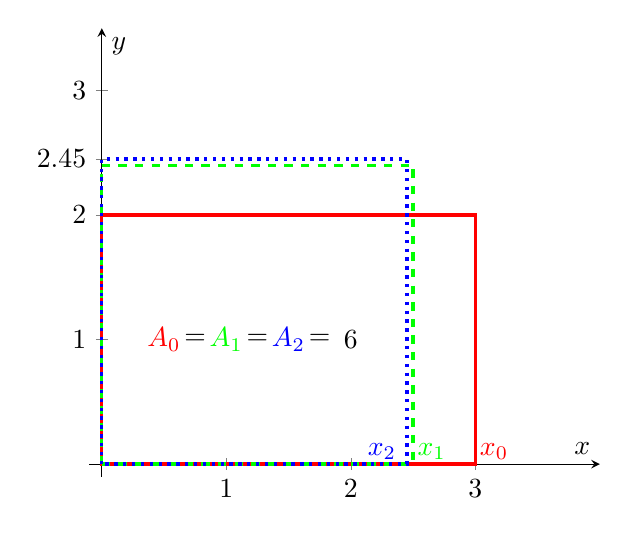
\begin{tikzpicture}
\begin{axis}[
    axis lines=middle,
    axis equal image,
    xlabel=$x$,
    ylabel=$y$,
    xmin=-0.1,xmax=4,
    ymin=-0.1,ymax=3.5,
    xtick={0, 1, 2, 3},
    ytick={0, 1, 2, 2.4494897427, 3},
]

    % iter 0
    \draw[very thick, red] (0, 0) rectangle (3, 2);
    \node[red] at (axis cs:3.15, 0.1) {$x_0$};

    % iter 1
    \draw[very thick, green, dashed] (0, 0) rectangle (2.5, 2.4);
    \node[green] at (axis cs:2.65, 0.1) {$x_1$};

    % iter 2
    \draw[very thick, blue,dotted] (0, 0) rectangle (2.45,	2.4489795918367343);
    \node[blue] at (axis cs:2.25, 0.1) {$x_2$};
    
    \node[red] at (axis cs:0.5, 1) {$A_0$};
    \node[green] at (axis cs:1, 1) {$A_1$};
    \node[blue] at (axis cs:1.5, 1) {$A_2$};
    \node at (axis cs:2, 1) {$6$};
    \node at (axis cs:0.75, 1) {$=$};
    \node at (axis cs:1.25, 1) {$=$};
    \node at (axis cs:1.75, 1) {$=$};


% \xdef\xold{3}
% \xdef\yold{2}
% \foreach \k in {0,...,2}{
%     \pgfmathsetmacro{\xnew}{(\xold + ((pow(\xold,2)-6) / \xold))/2}
%     \pgfmathsetmacro{\ynew}{6 / \xold}
%     \draw (0, 0) rectangle (\xold, \yold);

%     \global\let\xold\xnew
%     \global\let\yold\ynew
% }
\end{axis}
\end{tikzpicture}
\end{document}

Descrizione: Tre rettangoli equivalenti che approssimano un quadrato
Argomento sotteso: Metodo di Erone di Alessandria per il calcolo delle radici quadrate

Immagine che mostra il metodo (algoritmo) di Erone di Alessandria per il calcolo della radice quadrata di 6.

Informatica:
Derivare l'iterata x_{k+i} = 1/2 * (x_k + A/x_k) spiegando che il metodo di Erone approssima il lato di un quadrato partendo da una stima x_k, calcolando l'altezza del rettangolo di area data, e migliorando la stima come media aritmetica tra x_k e l'altezza A/x_k.

Mostrare che tale iterata è la stessa del metodo di Newton (delle tangenti).

Possibili collegamenti

Matematica: Derivazione.

Fisica: velocità istantanea, accelerazione istantanea...

Italiano: Futurismo

Storia: Prima Guerra Mondiale, Fascismo


Filosofia:  Concezione del tempo, tempo assoluto e relativo, oppure la velocità delle macchine e Marx, oppure concezione meccanicista del mondo.

Inglese: Poeti di guerra

Scienze: qualunque cosa che abbia a che fare con la velocità (tempo), ad esempio i catalizzatori